***REMOVED***
%% bare_jrnl.tex
%% V1.3
%% 2007/01/11
%% by Michael Shell
%% see http://www.michaelshell.org/
%% for current contact information.
%%
%% This is a skeleton file demonstrating the use of IEEEtran.cls
%% (requires IEEEtran.cls version 1.7 or later) with an IEEE journal paper.
%%
%% Support sites:
%% http://www.michaelshell.org/tex/ieeetran/
%% http://www.ctan.org/tex-archive/macros/latex/contrib/IEEEtran/
%% and
%% http://www.ieee.org/
***REMOVED***
***REMOVED***
***REMOVED***
% *** Authors should verify (and, if needed, correct) their LaTeX system  ***
% *** with the testflow diagnostic prior to trusting their LaTeX platform ***
% *** with production work. IEEE's font choices can trigger bugs that do  ***
% *** not appear when using other class files.                            ***
% The testflow support page is at:
% http://www.michaelshell.org/tex/testflow/
***REMOVED***
***REMOVED***
%%*************************************************************************
%% Legal Notice:
%% This code is offered as-is without any warranty either expressed or
%% implied; without even the implied warranty of MERCHANTABILITY or
%% FITNESS FOR A PARTICULAR PURPOSE! 
%% User assumes all risk.
%% In no event shall IEEE or any contributor to this code be liable for
%% any damages or losses, including, but not limited to, incidental,
%% consequential, or any other damages, resulting from the use or misuse
%% of any information contained here.
%%
%% All comments are the opinions of their respective authors and are not
%% necessarily endorsed by the IEEE.
%%
%% This work is distributed under the LaTeX Project Public License (LPPL)
%% ( http://www.latex-project.org/ ) version 1.3, and may be freely used,
%% distributed and modified. A copy of the LPPL, version 1.3, is included
%% in the base LaTeX documentation of all distributions of LaTeX released
%% 2003/12/01 or later.
%% Retain all contribution notices and credits.
%% ** Modified files should be clearly indicated as such, including  **
%% ** renaming them and changing author support contact information. **
%%
%% File list of work: IEEEtran.cls, IEEEtran_HOWTO.pdf, bare_adv.tex,
%%                    bare_conf.tex, bare_jrnl.tex, bare_jrnl_compsoc.tex
%%*************************************************************************
***REMOVED***
% Note that the a4paper option is mainly intended so that authors in
% countries using A4 can easily print to A4 and see how their papers will
% look in print - the typesetting of the document will not typically be
% affected with changes in paper size (but the bottom and side margins will).
% Use the testflow package mentioned above to verify correct handling of
% both paper sizes by the user's LaTeX system.
%
% Also note that the "draftcls" or "draftclsnofoot", not "draft", option
% should be used if it is desired that the figures are to be displayed in
% draft mode.
%
\documentclass[10pt, journal, twocolumn]{IEEEtran}
%
% If IEEEtran.cls has not been installed into the LaTeX system files,
% manually specify the path to it like:
% \documentclass[journal]{../sty/IEEEtran}
***REMOVED***
***REMOVED***
***REMOVED***
***REMOVED***
***REMOVED***
% Some very useful LaTeX packages include:
% (uncomment the ones you want to load)
***REMOVED***
***REMOVED***
% *** MISC UTILITY PACKAGES ***
%
%\usepackage{ifpdf}
% Heiko Oberdiek's ifpdf.sty is very useful if you need conditional
% compilation based on whether the output is pdf or dvi.
% usage:
% \ifpdf
%   % pdf code
% \else
%   % dvi code
% \fi
% The latest version of ifpdf.sty can be obtained from:
% http://www.ctan.org/tex-archive/macros/latex/contrib/oberdiek/
% Also, note that IEEEtran.cls V1.7 and later provides a builtin
% \ifCLASSINFOpdf conditional that works the same way.
% When switching from latex to pdflatex and vice-versa, the compiler may
% have to be run twice to clear warning/error messages.
***REMOVED***
***REMOVED***
***REMOVED***
***REMOVED***
***REMOVED***
***REMOVED***
% *** CITATION PACKAGES ***
%
%\usepackage{cite}
% cite.sty was written by Donald Arseneau
% V1.6 and later of IEEEtran pre-defines the format of the cite.sty package
% \cite{} output to follow that of IEEE. Loading the cite package will
% result in citation numbers being automatically sorted and properly
% "compressed/ranged". e.g., [1], [9], [2], [7], [5], [6] without using
% cite.sty will become [1], [2], [5]--[7], [9] using cite.sty. cite.sty's
% \cite will automatically add leading space, if needed. Use cite.sty's
% noadjust option (cite.sty V3.8 and later) if you want to turn this off.
% cite.sty is already installed on most LaTeX systems. Be sure and use
% version 4.0 (2003-05-27) and later if using hyperref.sty. cite.sty does
% not currently provide for hyperlinked citations.
% The latest version can be obtained at:
% http://www.ctan.org/tex-archive/macros/latex/contrib/cite/
% The documentation is contained in the cite.sty file itself.
***REMOVED***
***REMOVED***
***REMOVED***
***REMOVED***
***REMOVED***
***REMOVED***
% *** GRAPHICS RELATED PACKAGES ***
%
\ifCLASSINFOpdf
  \usepackage[pdftex]{graphicx}
  % declare the path(s) where your graphic files are
  % \graphicspath{{../pdf/}{../jpeg/}}
  % and their extensions so you won't have to specify these with
  % every instance of \includegraphics
  \DeclareGraphicsExtensions{.pdf,.jpeg,.png}
\else
  % or other class option (dvipsone, dvipdf, if not using dvips). graphicx
  % will default to the driver specified in the system graphics.cfg if no
  % driver is specified.
  \usepackage[dvips]{graphicx}
  % declare the path(s) where your graphic files are
  % \graphicspath{{../eps/}}
  % and their extensions so you won't have to specify these with
  % every instance of \includegraphics
  % \DeclareGraphicsExtensions{.eps}
\fi
% graphicx was written by David Carlisle and Sebastian Rahtz. It is
% required if you want graphics, photos, etc. graphicx.sty is already
% installed on most LaTeX systems. The latest version and documentation can
% be obtained at: 
% http://www.ctan.org/tex-archive/macros/latex/required/graphics/
% Another good source of documentation is "Using Imported Graphics in
% LaTeX2e" by Keith Reckdahl which can be found as epslatex.ps or
% epslatex.pdf at: http://www.ctan.org/tex-archive/info/
%
% latex, and pdflatex in dvi mode, support graphics in encapsulated
% postscript (.eps) format. pdflatex in pdf mode supports graphics
% in .pdf, .jpeg, .png and .mps (metapost) formats. Users should ensure
% that all non-photo figures use a vector format (.eps, .pdf, .mps) and
% not a bitmapped formats (.jpeg, .png). IEEE frowns on bitmapped formats
% which can result in "jaggedy"/blurry rendering of lines and letters as
% well as large increases in file sizes.
%
% You can find documentation about the pdfTeX application at:
% http://www.tug.org/applications/pdftex
***REMOVED***
***REMOVED***
***REMOVED***
***REMOVED***
***REMOVED***
% *** MATH PACKAGES ***
%
\usepackage[cmex10]{amsmath}
% A popular package from the American Mathematical Society that provides
% many useful and powerful commands for dealing with mathematics. If using
% it, be sure to load this package with the cmex10 option to ensure that
% only type 1 fonts will utilized at all point sizes. Without this option,
% it is possible that some math symbols, particularly those within
% footnotes, will be rendered in bitmap form which will result in a
% document that can not be IEEE Xplore compliant!
%
% Also, note that the amsmath package sets \interdisplaylinepenalty to 10000
% thus preventing page breaks from occurring within multiline equations. Use:
%\interdisplaylinepenalty=2500
% after loading amsmath to restore such page breaks as IEEEtran.cls normally
% does. amsmath.sty is already installed on most LaTeX systems. The latest
% version and documentation can be obtained at:
% http://www.ctan.org/tex-archive/macros/latex/required/amslatex/math/
***REMOVED***
***REMOVED***
***REMOVED***
***REMOVED***
***REMOVED***
% *** SPECIALIZED LIST PACKAGES ***
%
%\usepackage{algorithmic}
% algorithmic.sty was written by Peter Williams and Rogerio Brito.
% This package provides an algorithmic environment fo describing algorithms.
% You can use the algorithmic environment in-text or within a figure
% environment to provide for a floating algorithm. Do NOT use the algorithm
% floating environment provided by algorithm.sty (by the same authors) or
% algorithm2e.sty (by Christophe Fiorio) as IEEE does not use dedicated
% algorithm float types and packages that provide these will not provide
% correct IEEE style captions. The latest version and documentation of
% algorithmic.sty can be obtained at:
% http://www.ctan.org/tex-archive/macros/latex/contrib/algorithms/
% There is also a support site at:
% http://algorithms.berlios.de/index.html
% Also of interest may be the (relatively newer and more customizable)
% algorithmicx.sty package by Szasz Janos:
% http://www.ctan.org/tex-archive/macros/latex/contrib/algorithmicx/
***REMOVED***
***REMOVED***
***REMOVED***
***REMOVED***
% *** ALIGNMENT PACKAGES ***
%
%\usepackage{array}
% Frank Mittelbach's and David Carlisle's array.sty patches and improves
% the standard LaTeX2e array and tabular environments to provide better
% appearance and additional user controls. As the default LaTeX2e table
% generation code is lacking to the point of almost being broken with
% respect to the quality of the end results, all users are strongly
% advised to use an enhanced (at the very least that provided by array.sty)
% set of table tools. array.sty is already installed on most systems. The
% latest version and documentation can be obtained at:
% http://www.ctan.org/tex-archive/macros/latex/required/tools/
***REMOVED***
***REMOVED***
%\usepackage{mdwmath}
%\usepackage{mdwtab}
% Also highly recommended is Mark Wooding's extremely powerful MDW tools,
% especially mdwmath.sty and mdwtab.sty which are used to format equations
% and tables, respectively. The MDWtools set is already installed on most
% LaTeX systems. The lastest version and documentation is available at:
% http://www.ctan.org/tex-archive/macros/latex/contrib/mdwtools/
***REMOVED***
***REMOVED***
% IEEEtran contains the IEEEeqnarray family of commands that can be used to
% generate multiline equations as well as matrices, tables, etc., of high
% quality.
***REMOVED***
***REMOVED***
%\usepackage{eqparbox}
% Also of notable interest is Scott Pakin's eqparbox package for creating
% (automatically sized) equal width boxes - aka "natural width parboxes".
% Available at:
% http://www.ctan.org/tex-archive/macros/latex/contrib/eqparbox/
***REMOVED***
***REMOVED***
***REMOVED***
***REMOVED***
***REMOVED***
% *** SUBFIGURE PACKAGES ***
%\usepackage[tight,footnotesize]{subfigure}
% subfigure.sty was written by Steven Douglas Cochran. This package makes it
% easy to put subfigures in your figures. e.g., "Figure 1a and 1b". For IEEE
% work, it is a good idea to load it with the tight package option to reduce
% the amount of white space around the subfigures. subfigure.sty is already
% installed on most LaTeX systems. The latest version and documentation can
% be obtained at:
% http://www.ctan.org/tex-archive/obsolete/macros/latex/contrib/subfigure/
% subfigure.sty has been superceeded by subfig.sty.
***REMOVED***
***REMOVED***
***REMOVED***
%\usepackage[caption=false]{caption}
%\usepackage[font=footnotesize]{subfig}
% subfig.sty, also written by Steven Douglas Cochran, is the modern
% replacement for subfigure.sty. However, subfig.sty requires and
% automatically loads Axel Sommerfeldt's caption.sty which will override
% IEEEtran.cls handling of captions and this will result in nonIEEE style
% figure/table captions. To prevent this problem, be sure and preload
% caption.sty with its "caption=false" package option. This is will preserve
% IEEEtran.cls handing of captions. Version 1.3 (2005/06/28) and later 
% (recommended due to many improvements over 1.2) of subfig.sty supports
% the caption=false option directly:
%\usepackage[caption=false,font=footnotesize]{subfig}
%
% The latest version and documentation can be obtained at:
% http://www.ctan.org/tex-archive/macros/latex/contrib/subfig/
% The latest version and documentation of caption.sty can be obtained at:
% http://www.ctan.org/tex-archive/macros/latex/contrib/caption/
***REMOVED***
***REMOVED***
***REMOVED***
***REMOVED***
% *** FLOAT PACKAGES ***
%
%\usepackage{fixltx2e}
% fixltx2e, the successor to the earlier fix2col.sty, was written by
% Frank Mittelbach and David Carlisle. This package corrects a few problems
% in the LaTeX2e kernel, the most notable of which is that in current
% LaTeX2e releases, the ordering of single and double column floats is not
% guaranteed to be preserved. Thus, an unpatched LaTeX2e can allow a
% single column figure to be placed prior to an earlier double column
% figure. The latest version and documentation can be found at:
% http://www.ctan.org/tex-archive/macros/latex/base/
***REMOVED***
***REMOVED***
***REMOVED***
%\usepackage{stfloats}
% stfloats.sty was written by Sigitas Tolusis. This package gives LaTeX2e
% the ability to do double column floats at the bottom of the page as well
% as the top. (e.g., "\begin{figure*}[!b]" is not normally possible in
% LaTeX2e). It also provides a command:
%\fnbelowfloat
% to enable the placement of footnotes below bottom floats (the standard
% LaTeX2e kernel puts them above bottom floats). This is an invasive package
% which rewrites many portions of the LaTeX2e float routines. It may not work
% with other packages that modify the LaTeX2e float routines. The latest
% version and documentation can be obtained at:
% http://www.ctan.org/tex-archive/macros/latex/contrib/sttools/
% Documentation is contained in the stfloats.sty comments as well as in the
% presfull.pdf file. Do not use the stfloats baselinefloat ability as IEEE
% does not allow \baselineskip to stretch. Authors submitting work to the
% IEEE should note that IEEE rarely uses double column equations and
% that authors should try to avoid such use. Do not be tempted to use the
% cuted.sty or midfloat.sty packages (also by Sigitas Tolusis) as IEEE does
% not format its papers in such ways.
***REMOVED***
***REMOVED***
%\ifCLASSOPTIONcaptionsoff
%  \usepackage[nomarkers]{endfloat}
% \let\MYoriglatexcaption\caption
% \renewcommand{\caption}[2][\relax]{\MYoriglatexcaption[#2]{#2}}
%\fi
% endfloat.sty was written by James Darrell McCauley and Jeff Goldberg.
% This package may be useful when used in conjunction with IEEEtran.cls'
% captionsoff option. Some IEEE journals/societies require that submissions
% have lists of figures/tables at the end of the paper and that
% figures/tables without any captions are placed on a page by themselves at
% the end of the document. If needed, the draftcls IEEEtran class option or
% \CLASSINPUTbaselinestretch interface can be used to increase the line
% spacing as well. Be sure and use the nomarkers option of endfloat to
% prevent endfloat from "marking" where the figures would have been placed
% in the text. The two hack lines of code above are a slight modification of
% that suggested by in the endfloat docs (section 8.3.1) to ensure that
% the full captions always appear in the list of figures/tables - even if
% the user used the short optional argument of \caption[]{}.
% IEEE papers do not typically make use of \caption[]'s optional argument,
% so this should not be an issue. A similar trick can be used to disable
% captions of packages such as subfig.sty that lack options to turn off
% the subcaptions:
% For subfig.sty:
% \let\MYorigsubfloat\subfloat
% \renewcommand{\subfloat}[2][\relax]{\MYorigsubfloat[]{#2}}
% For subfigure.sty:
% \let\MYorigsubfigure\subfigure
% \renewcommand{\subfigure}[2][\relax]{\MYorigsubfigure[]{#2}}
% However, the above trick will not work if both optional arguments of
% the \subfloat/subfig command are used. Furthermore, there needs to be a
% description of each subfigure *somewhere* and endfloat does not add
% subfigure captions to its list of figures. Thus, the best approach is to
% avoid the use of subfigure captions (many IEEE journals avoid them anyway)
% and instead reference/explain all the subfigures within the main caption.
% The latest version of endfloat.sty and its documentation can obtained at:
% http://www.ctan.org/tex-archive/macros/latex/contrib/endfloat/
%
% The IEEEtran \ifCLASSOPTIONcaptionsoff conditional can also be used
% later in the document, say, to conditionally put the References on a 
% page by themselves.
***REMOVED***
***REMOVED***
***REMOVED***
***REMOVED***
***REMOVED***
% *** PDF, URL AND HYPERLINK PACKAGES ***
%
%\usepackage{url}
% url.sty was written by Donald Arseneau. It provides better support for
% handling and breaking URLs. url.sty is already installed on most LaTeX
% systems. The latest version can be obtained at:
% http://www.ctan.org/tex-archive/macros/latex/contrib/misc/
% Read the url.sty source comments for usage information. Basically,
% \url{my_url_here}.
***REMOVED***
***REMOVED***
***REMOVED***
***REMOVED***
***REMOVED***
% *** Do not adjust lengths that control margins, column widths, etc. ***
% *** Do not use packages that alter fonts (such as pslatex).         ***
% There should be no need to do such things with IEEEtran.cls V1.6 and later.
% (Unless specifically asked to do so by the journal or conference you plan
% to submit to, of course. )
***REMOVED***
***REMOVED***
% Paket für Anmerkungen an der Seite
\usepackage{marginnote}
\usepackage{amsfonts}
***REMOVED***
***REMOVED***
% correct bad hyphenation here
\hyphenation{op-tical net-works semi-conduc-tor}
***REMOVED***
% Big 0 Notation
\newcommand{\BigO}[1]{\ensuremath{\operatorname{O}\bigl(#1\bigr)}}
***REMOVED***
%\usepackage{float}
%\usepackage{multicol-floats}
%\floatstyle{boxed} % Box...
%\restylefloat{figure}% ...figure environment contents.
***REMOVED***
\begin{document}
%
% paper title
% can use linebreaks \\ within to get better formatting as desired
\title{Data Model Analysis Of Database Schemes For Enterprise Software Systems}
%
%
% author names and IEEE memberships
% note positions of commas and nonbreaking spaces ( ~ ) LaTeX will not break
% a structure at a ~ so this keeps an author's name from being broken across
% two lines.
% use \thanks{} to gain access to the first footnote area
% a separate \thanks must be used for each paragraph as LaTeX2e's \thanks
% was not built to handle multiple paragraphs
%
***REMOVED***
\author{Danijar Hafner \& Jakob Frick\\Tutor: Martin Lorenz\\Hasso Plattner Institut}% <-this % stops a space
***REMOVED***
% The paper headers
\markboth{Enterprise Software Systems: Programming Concepts and Application Characteristics}{}
% The only time the second header will appear is for the odd numbered pages
% after the title page when using the twoside option.
% 
% *** Note that you probably will NOT want to include the author's ***
% *** name in the headers of peer review papers.                   ***
% You can use \ifCLASSOPTIONpeerreview for conditional compilation here if
% you desire.
***REMOVED***
***REMOVED***
***REMOVED***
***REMOVED***
% If you want to put a publisher's ID mark on the page you can do it like
% this:
%\IEEEpubid{0000--0000/00\$00.00~\copyright~2007 IEEE}
% Remember, if you use this you must call \IEEEpubidadjcol in the second
% column for its text to clear the IEEEpubid mark.
***REMOVED***
***REMOVED***
***REMOVED***
% use for special paper notices
%\IEEEspecialpapernotice{(Invited Paper)}
***REMOVED***
***REMOVED***
***REMOVED***
***REMOVED***
% make the title area
\maketitle
***REMOVED***
***REMOVED***
\begin{abstract}
%\boldmath
The abstract goes here.
\end{abstract}
% IEEEtran.cls defaults to using nonbold math in the Abstract.
% This preserves the distinction between vectors and scalars. However,
% if the journal you are submitting to favors bold math in the abstract,
% then you can use LaTeX's standard command \boldmath at the very start
% of the abstract to achieve this. Many IEEE journals frown on math
% in the abstract anyway.
***REMOVED***
% Note that keywords are not normally used for peerreview papers.
\begin{IEEEkeywords}
IEEEtran, journal, \LaTeX, paper, template.
\end{IEEEkeywords}
***REMOVED***
***REMOVED***
***REMOVED***
***REMOVED***
***REMOVED***
***REMOVED***
% For peer review papers, you can put extra information on the cover
% page as needed:
% \ifCLASSOPTIONpeerreview
% \begin{center} \bfseries EDICS Category: 3-BBND \end{center}
% \fi
%
% For peerreview papers, this IEEEtran command inserts a page break and
% creates the second title. It will be ignored for other modes.
\IEEEpeerreviewmaketitle
***REMOVED***
***REMOVED***
***REMOVED***
\section{Introduction}
% The very first letter is a 2 line initial drop letter followed
% by the rest of the first word in caps.
% 
% form to use if the first word consists of a single letter:
% \IEEEPARstart{A}{demo} file is ....
% 
% form to use if you need the single drop letter followed by
% normal text (unknown if ever used by IEEE):
% \IEEEPARstart{A}{}demo file is ....
% 
% Some journals put the first two words in caps:
% \IEEEPARstart{T}{his demo} file is ....
% 
% Here we have the typical use of a "T" for an initial drop letter
% and "HIS" in caps to complete the first word.
\IEEEPARstart{E}{nterprise} Software has nowadays become one of the most complex and difficult fields of software engineering. Enterprise Software not only has to fulfill various types of task and challenges, but has also to work flawless and efficient. In advance one enterprise software is often used in different branches and divisions and has an code base which has grown over time. Therefore the code base of an enterprise software and the database scheme of the software backed have become confusing and hard to manage. The aim of this paper is to present an algorithm, which tackles these problems. Based on a peer-to-peer comparison of database tables of an ERP system the algorithm builds up an hierarchy of inheritance and identifies certain clusters of connected tables. To do so the algorithm tries to identify inheritance relations among the tables and bring them in order. The output is a set of cluster, which themselves are organized as trees of tables. Besides the algorithm this paper discusses also certain patterns, which can be found in the clusters and can be seen as certain steps of development in the database scheme.  
% You must have at least 2 lines in the paragraph with the drop letter
% (should never be an issue) 
%I wish you the best of success.
***REMOVED***
%\hfill mds
 
%\hfill January 11, 2007
***REMOVED***
\subsection{Subsection Heading Here}
Subsection text here.
***REMOVED***
% needed in second column of first page if using \IEEEpubid
%\IEEEpubidadjcol
***REMOVED***
\subsubsection{Subsubsection Heading Here}
Subsubsection text here.
***REMOVED***
***REMOVED***
% An example of a floating figure using the graphicx package.
% Note that \label must occur AFTER (or within) \caption.
% For figures, \caption should occur after the \includegraphics.
% Note that IEEEtran v1.7 and later has special internal code that
% is designed to preserve the operation of \label within \caption
% even when the captionsoff option is in effect. However, because
% of issues like this, it may be the safest practice to put all your
% \label just after \caption rather than within \caption{}.
%
% Reminder: the "draftcls" or "draftclsnofoot", not "draft", class
% option should be used if it is desired that the figures are to be
% displayed while in draft mode.
%
%\begin{figure}[!t]
%\centering
%\includegraphics[width=2.5in]{myfigure}
% where an .eps filename suffix will be assumed under latex, 
% and a .pdf suffix will be assumed for pdflatex; or what has been declared
% via \DeclareGraphicsExtensions.
%\caption{Simulation Results}
%\label{fig_sim}
%\end{figure}
***REMOVED***
% Note that IEEE typically puts floats only at the top, even when this
% results in a large percentage of a column being occupied by floats.
***REMOVED***
***REMOVED***
% An example of a double column floating figure using two subfigures.
% (The subfig.sty package must be loaded for this to work.)
% The subfigure \label commands are set within each subfloat command, the
% \label for the overall figure must come after \caption.
% \hfil must be used as a separator to get equal spacing.
% The subfigure.sty package works much the same way, except \subfigure is
% used instead of \subfloat.
%
%\begin{figure*}[!t]
%\centerline{\subfloat[Case I]\includegraphics[width=2.5in]{subfigcase1}%
%\label{fig_first_case}}
%\hfil
%\subfloat[Case II]{\includegraphics[width=2.5in]{subfigcase2}%
%\label{fig_second_case}}}
%\caption{Simulation results}
%\label{fig_sim}
%\end{figure*}
%
% Note that often IEEE papers with subfigures do not employ subfigure
% captions (using the optional argument to \subfloat), but instead will
% reference/describe all of them (a), (b), etc., within the main caption.
***REMOVED***
***REMOVED***
% An example of a floating table. Note that, for IEEE style tables, the 
% \caption command should come BEFORE the table. Table text will default to
% \footnotesize as IEEE normally uses this smaller font for tables.
% The \label must come after \caption as always.
%
%\begin{table}[!t]
%% increase table row spacing, adjust to taste
%\renewcommand{\arraystretch}{1.3}
% if using array.sty, it might be a good idea to tweak the value of
% \extrarowheight as needed to properly center the text within the cells
%\caption{An Example of a Table}
%\label{table_example}
%\centering
%% Some packages, such as MDW tools, offer better commands for making tables
%% than the plain LaTeX2e tabular which is used here.
%\begin{tabular}{|c||c|}
%\hline
%One & Two\\
%\hline
%Three & Four\\
%\hline
%\end{tabular}
%\end{table}
***REMOVED***
***REMOVED***
% Note that IEEE does not put floats in the very first column - or typically
% anywhere on the first page for that matter. Also, in-text middle ("here")
% positioning is not used. Most IEEE journals use top floats exclusively.
% Note that, LaTeX2e, unlike IEEE journals, places footnotes above bottom
% floats. This can be corrected via the \fnbelowfloat command of the
% stfloats package.
***REMOVED***
***REMOVED***
***REMOVED***
\section{The input data}
\IEEEPARstart{T}{he} algorithm works on a set of peer-to-peer compares of tables in a database scheme. The input data need the following characteristics to work with the algorithm: Be $S$ the database scheme and $T_a$, $T_b$ tables from this scheme, so has the input data the following character 
$$\{T_a, T_b \in S | (T_a, T_b, \delta_{parent\_ratio}(T_a, T_b),\delta_{child\_ratio}(T_a, T_b))\}$$\hspace{-300cm} 
.\footnote{Überprüfen ob das nur ein beispiel für parent child ratio ist. eventuell mit tobi + alex absprechen, vielleicht sonst einfach als naives beispiel angeben} Whereby the $\delta_{parent\_ratio}(T_a, T_b)$ and $\delta_{child\_ratio}(T_a, T_b))$ are calculated by the following formula: $$\delta_{parent\_ratio}(T_a, T_b) = \frac{ | T_a \cap T_b |}{ | T_a |} $$ and  $$\delta_{child\_ratio}(T_a, T_b) = \frac{ | T_a \cap T_b |}{ | T_b |} $$\\
(Note that by $| T_a |$ the amount of fields in $T_a$ is meant and that $T_a \cap T_b$ are all fields, which $T_a$ and $T_b$ have in common)\\
\\Conclusion:
\begin{itemize}
\item Each of the tuples is a statement about how similar two tables are, characterized by the amount of fields they have in common. 
\item $\delta_{parent\_ratio}$ means how much a parent - the first element of the tuple - is in the child - the second element of the tuple - and vice versa for $\delta_{child\_ratio}$.
\end{itemize}
Be aware that parent and child in this context are only statement about the order in the compare not yet and actual statement about an inheritance relation between $T_a$ and $T_b$.\\
\\For an example of how such data can be generated from a database scheme see Kastius\&Nack \footnote{VERWEIS AUF ALEX+TOBIS PAPER}.\\
Advice: To fasten the algorithm it might come in handy to define a threshold for the compares. This threshold could be defined by the median of $\delta_{parent\_ratio}$ and $\delta_{child\_ratio}$ and can be used to sort out lose connections, which become irrelevant for the data analysis. For example: Be threshold $$ \tau = 0.8$$ then $input$ will only consist out of compares, which fulfill the following equation: $$ \tau < \frac{\delta_{parent\_ratio} +  \delta_{child\_ratio}}{2} $$ $\Leftrightarrow$ $$0.8 < \frac{\delta_{parent\_ratio} +  \delta_{child\_ratio}}{2} $$
***REMOVED***
Example: \footnote{Hier hier noch ein beispiel??}
\section{The algorithm}
\IEEEPARstart{A}{fter} generating or fetching input data in the certain format the algorithm can work. It operates in certain steps: \begin{enumerate}
\item Preprocessing
\begin{enumerate}
\item Summarizing copies
\item Identifying parents
\end{enumerate}
\item Building a hierarchy
\item Postprocessing
\begin{enumerate}
\item Calculating amounts 
\item Calculating differences
\end{enumerate}
\end{enumerate}
***REMOVED***
\subsection{Preprocessing}
Based on the input data the algorithm builds up an mapping from ids to a sets of tables. Each relation is processed and checked, if for any of the two tables in the relation an id was not assigned yet. If so a new id is created and a mapping from this id to a new set, with the table as single element, is saved. \\
\subsubsection{Summarizing copies}
In the same step the algorithm notices copies of tables. These can easy identified by parent and child ratio. Because the following formula applies: $$ T_a \cap T_b = T_a = T_b$$ $$\Rightarrow \delta_{parent\_ratio} =  \delta_{child\_ratio} = 1.0$$
If a copy is found the two identical tables are saved in a common set under the same id. Because the algorithm in the following steps only processes ids. copies are therefore handled as one distinct table and not processed multiple times. It is important that in the post processing the mapping from ids to multiple tables is correctly exported and displayed.\\
\textbf{Note:} This way of summarizing copies could create several clusters, which are in fact copies among themselves through transitive relations. To avoid this problem either a \textit{connected component finding} algorithm has to be used or the input data has to be sorted, when fetched. If the data is sorted by $T_a$,$\delta_{parent\_ratio}$,$\delta_{child\_ratio}$ this ensures that transitional relations are processed in order and sets of copies are disjoint.\\
\\\subsubsection{Identifying parents}
After each distinct table has been identified, the relations from the input data are represented in a mapping ($f\_ratio$) from table id to table id with the parent ratio: $$f\_ratio: S^{2} \rightarrow \mathbb{R}$$ $$T_a, T_b \in S: f\_ratio(T_a, T_b) = \delta_{parent\_ratio}(T_a,T_b)$$ .  Keep in mind that every tuple from the input data is an information about how similar two tables are. In fact the map of the relations can be seen as a representation of a directed graph, where the different tables are the nodes and the relations are directed edges.\footnote{grafik wäre schön :) } This mapping/graph is the foundation for the fast and efficient identification of the parent and the children in the inheritance relations. Therefore unnecessary edges have to be removed, so that each node has only one edge, which directs to its parent. The nodes with no connection to another parent can be seen as \textit{cluster parents} and are the \textbf{root}s for an inheritance tree with all the tables that have inherited from this \textit{cluster parent}. All inheritance trees with their respective root parents can be seen as disjoint \textbf{clusters}.
This structure is achieved by the following algorithm, which is done for all distinct tables: \begin{enumerate}
\item Choose a table $T_{cur}$ to be processed: $$T_{cur} \in S \wedge \exists T_{other} \in S: (T_{cur}, T_{other}) \in domain(f\_ratio)$$
\item Find the table $T_{par}$ which has the highest parent ratio for the $T_{cur}$: $$T_{par}, \forall T_{o}: f\_ratio(T_o, T_{cur}) < f\_ratio(T_{par},T_{cur}) $$
\item Now $f\_ratio(T_{par},T_{cur})$ has to be compared with the reverse connection $f\_ratio(T_{cur},T_{par})$ (if existing):
\begin{enumerate}
\item If $f\_ratio(T_{par},T_{cur}) > f\_ratio(T_{cur},T_{par})$ is true, the new connection has to be saved in a mapping from parent to child: $$f\_children: S \rightarrow S^*$$, which gives for each parent table a set of it children.
\item If $f\_ratio(T_{par},T_{cur}) < f\_ratio(T_{cur},T_{par})$ is true, the connection is actually the other way around and $T_{cur}$ is a parent for $T_{par}$. Furthermore $T_{cur}$ is a cluster parent because it has no parent.
\end{enumerate}
\end{enumerate}
With this processing every node has either a distinct parent node or is a cluster root node. Because the identification of the parent node is based only on $\delta_{parent\_ratio}$ its quality depends very much on the quality of $\delta_{parent\_ratio}$. 
\\\subsection{Building a hierarchy}
In the preprocessing a mapping was created, which gives for every distinct table a set of its children ($f\_ch$), and the root nodes for the clusters identified. This itself represents already the complete internal structure of the database scheme. To obtain an overall structure of a clusters, it must only be traversed recursively with $f\_ch$ starting at the respective root node. In addition the structure has also to be saved in a suited format, for example XML. Cluster, which consists out of only one table, can often be filtered out because there are irrelevant for a analysis of clusters and their inner structure. 
\\\subsection{Postprocessing}
After the structure of the cluster was build up as described above, some important figures can be calculated for the clusters, which than can be used to analyze the data afterwords:
\\\subsubsection{Calculation of the amounts}
To get the size of a cluster and the amount of tables, which direct and indirect inherited from a certain parent table, at first a mapping from table to the amount of its children has build. This can easily be done by using $f\_ch$: $$ f\_cham: S \rightarrow \mathbb{N} $$ $$T \in domain(f\_children): f\_cham(T) = | f\_ch(T) | $$\\
Now the size of each inheritance tree, where a certain table $T_{root}$ is the root node, can be calculated with a recursive, dynamic function:
$$ f\_am: S \rightarrow \mathbb{N} $$
$$ T \in domain(f\_children): $$ $$f\_am(T) = | f\_cham(T) | + \sum_{child \in f\_ch(T)}{f\_am(child)} $$
For the size of a whole cluster just $f\_amount$ of the root node has to be calculated.
\\\subsubsection{Calculation of the differences}
To enable an in-deep analysis of the single relations between two tables, for each relation a compare of the fields is computed. Therefore for every of the both tables in the relation the table structure is retrieved from the database system and compared. Now the added and removed fields from parent to child are saved in new mappings:
\begin{itemize}
\item In $$added: S \rightarrow Fields^*$$ a set of added fields is mapped to a certain child table. This mapping is distinct because for each child table, the parent table is distinct and therefore the child-parent relation.
\item In $$removed: S \rightarrow Fields^*$$ a set of removed fields is mapped to a certain child table. 
\end{itemize}
All three structures, $added$, $removed$ and $f\_amount$, can afterwards be used to make a statistic analysis of the cluster and to point out certain patterns in the inheritance structures of the clusters.
\subsection{Result}
As a result overall algorithm builds up and returns the following structures:
\begin{itemize}
\item $f\_children$: A mapping from a table to a set of its children.
\item $f\_childrenamount$: A mapping from a table to the amount of its children.
\item $f\_amount$: A mapping from a table to the amount of tables in the from it outgoing inheritance tree.
\item $added$: A mapping from a table to a set of the fields, that were added from it's parent table to itself.
\item $removed$: A mapping from a table to a set of the fields, that were removed from it's parent table to itself.
\end{itemize}
\subsection{Runtime analysis}
Also a runtime analysis of the algorithm can be easily done, by analyzing the different steps of the algorithm:\\($n$ be the amount of relations in the input data, $p$ be the amount of parent nodes found in the cluster and $r$ be the amount of relations in the graph)
\begin{enumerate}
\item Summarizing copies and creating id mapping: \BigO{n}
\item Identifying parents: \BigO{n*1/log(n)} \footnote{zu ueberpruefen}
\item Calculation the amount children: \BigO{p}
\item Calculation the amount of nodes in the clusters (with caching): \BigO{p}
\item Calculation of added and removed: \BigO{2r}
\end{enumerate}
Because of $p \le r < n$ applies the overall runtime is about $ t \in $ \BigO{n* (1+ )}
***REMOVED***
\section{Advantages and shortcomings}
\subsection{Advantages}
\IEEEPARstart{T}{he} algorithm has some advantages, when it comes to analyze and characterize huge amount of tables and relations among them. The runtime complexity is low compared to some more common clustering algorithms like k-means. Furthermore the output can be used to easily analyze the database scheme for a widespread set of task and request. Copies of tables are detected early in the process and handled as one table and in the end the assignment of different tables to the cluster is very clear. But the key advantage of this algorithm is that it runs on any kind of comparison between database tables if an input data can be generated, which fulfills the described format.
\subsection{Shortcomings}
One of the biggest shortcomings of the algorithm is that it mostly depends on the quality of the input data. Because the algorithm has to build up on already made compares of the tables there is no way of ensure a correct clustering, if it has not been ensured for the input data. Therefore it should not be used for raw, unchecked input data. but the input should have been sanity-checked before applying the algorithm. Another problem is that in its current state the algorithm identifies only one parent of a certain table. It might be needed and reasonable to check, if a table has more than one parent even though this would add much more complexity to the algorithm, because it has to be ensured, that a another child from the same parent is not identified as other parent, just because of its similarity. Here again the algorithm relies on the input data. And in some scenarios the fact that the algorithm creates disjoint clusters could become a disadvantage because sometimes you might have tables, which originated from more than one \textit{cluster parent}.
\section{Patterns and statistics of example data}
\IEEEPARstart{T}{ested} on input set from an example database scheme off an ERP system, some characteristic patterns and relations between the tables were found several times. Also some interesting insights about the structure was gained.
\subsection{Characteristics of the sample data}
 anzahl der tabellen anzahl der vergleiche threshold bla bla bla blab
\subsection{Patterns}
\IEEEPARstart{T}here is a wide set of patterns in the relationships between the tables, which can be found several times throughout different clusters. The following patterns can be seen as an example of different steps a evolution of a database table. These steps are often modifications or changes that are not possible\footnote{hoert sich seltsam an} to the object-oriented model. The patterns where only analyzed between a parent table and it's respective children.
\subsubsection{Inheritance:}
\begin{figure}[h]
\centering
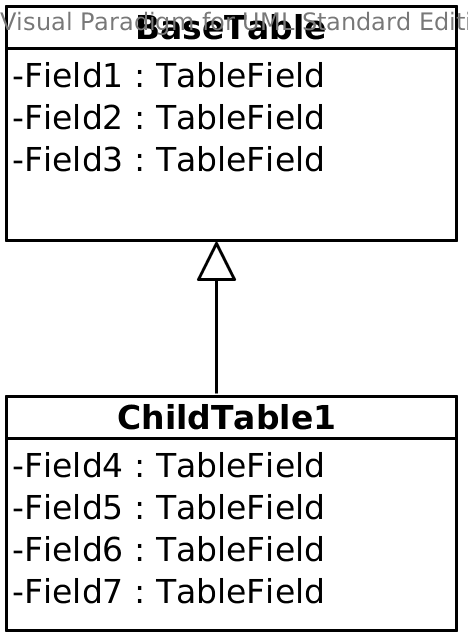
\includegraphics[width=1.5in]{SingleInheritance}
\caption{Schema of single inheritance}
\footnote{Hier die das UML Model}
\end{figure}
The most basic change between two tables is inheritance. This means that the child table consists out of the parent table but has additional table fields. It fits the inheritance relation known from the object-oriented model.
\begin{figure}[h]
\centering
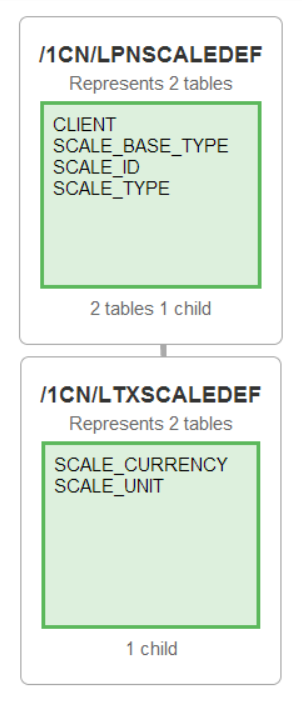
\includegraphics[width=1in]{SingleInheritance_ex}
\caption{Example of a single inheritance}
\footnote{Hier die Beispiel, bei allen anderen gleiches schema}
\end{figure}
\subsubsection{Multiple inheritance:}
Inheritance often occurs multiple times in one level of the cluster hierarchy. The parent table is used as a template for all its children and all these children share all the tables of the parent table. This is one of the clearest relations about how tables in one level of a cluster are connected. Especially small clusters with often are purely made of multiple or single inheritance.
\subsubsection{Modification:}
Modification is a pattern that is not possible in the common object-oriented model. A modification occurs in the relation between a parent and a child table, when the child not only has additional table fields but also misses some fields of the parent.
\subsubsection{Renaming:}
A renaming occurs when in the child table a certain table field was removed and is replaced by another, which has a different name but has an identical or similar domain name and data type. This often occurs multiple times in one level or step of a cluster and is an indicator that a table was used in a different context and therefore the field names had to been altered.
\subsubsection{Implicit base table:}
It occurs in the clusters that in one level it seems like a step or an base table is missing. This assumption can be drawn from the fact that all children tables in one level share a certain modification (addition and removing of table fields) compared to their respective base table, but a table with this certain modification is not in the input set. Therefore it can be concluded that in the modification of the children table from the base table, they all shared a certain prepossessing for which the result was not saved in the database.
\section{Statistic:}
For an example input set this characteristic was found:
\footnote{Hier noch mal alle statistik die wir haben, charts, charts, charts :D }
***REMOVED***
\section{Example deployment}
For the example analysis the following deployment environment was used:\footnote{hier noch ein deployment diagramm}
\begin{itemize}
\item The algorithm was implemented in a C++ program. This program fetched the input data from a HANA database and processed it in the described way.
\item The result mapping was written into a complete normalized database structure in the HANA database so it could be processed by external tools.
\item A Java Servlet running on an Apache Tomcat server was used a data distributor, which delivered for a table the joined results as JSON data via a REST-full interface.
\item The visualization was done by a single-page application implemented in Javascript, which lazy-loaded the data from the Java Servlet and made it possible to discover the hierarchy of the data interactive.
\end{itemize}
\footnote{Hier noch das Deploymentdiagram }
\section{Summary}
This paper describes an algorithm to analyze and categorize relations between tables in a database. The algorithm builds up on single relationships between the tables and builds up a set of distinct clusters. Each of the clusters has a tree hierarchy between the tables which is generated according to the input relations. The cluster are distinct and each has root table from which a chain of modification can be build up to any other table in the cluster. The clusters and the modifications between any root table and it's leafs are the output of this algorithm. They can be the foundation for further and more specific analysis of the table relations. Because the input data is only a set of relations between certain entities the algorithm can be used in a wide range of settings and applications.
\section{Further use and development}
Further development of the algorithm could include steps to detect inheritance from several parents and connections between the cluster as discussed above. Also a detection and inclusion of \textit{abstract parents}, as seen in \textit{Patterns} could be implemented. \\ In further projects the algorithm could be used together with statistics about the use of certain tables in a database scheme to rethink and restructure of certain aspects of the database scheme, to make it more efficient and reduce copies. Furthermore several patterns in a cluster or in the database system could be analyzed with an expert of this system, to make statements about the historic development of the system and to gain knowledge about how a further development can be shaped to improve the overall system.
% if have a single appendix:
%\appendix[Proof of the Zonklar Equations]
% or
%\appendix  % for no appendix heading
% do not use \section anymore after \appendix, only \section*
% is possibly needed
***REMOVED***
% use appendices with more than one appendix
% then use \section to start each appendix
% you must declare a \section before using any
% \subsection or using \label (\appendices by itself
% starts a section numbered zero.)
%
***REMOVED***
% Brauchen wir vielleicht noch
\appendices
\section{Proof of the First Zonklar Equation}
Hier noch zeug was wir eventuell bruachen
Appendix one text goes here.
***REMOVED***
% you can choose not to have a title for an appendix
% if you want by leaving the argument blank
\section{}
Appendix two text goes here.
***REMOVED***
***REMOVED***
% use section* for acknowledgement
\section*{Acknowledgment}
***REMOVED***
***REMOVED***
The authors would like to thank...
***REMOVED***
***REMOVED***
% Can use something like this to put references on a page
% by themselves when using endfloat and the captionsoff option.
\ifCLASSOPTIONcaptionsoff
  \newpage
\fi
***REMOVED***
***REMOVED***
***REMOVED***
% trigger a \newpage just before the given reference
% number - used to balance the columns on the last page
% adjust value as needed - may need to be readjusted if
% the document is modified later
%\IEEEtriggeratref{8}
% The "triggered" command can be changed if desired:
%\IEEEtriggercmd{\enlargethispage{-5in}}
***REMOVED***
% references section
***REMOVED***
% can use a bibliography generated by BibTeX as a .bbl file
% BibTeX documentation can be easily obtained at:
% http://www.ctan.org/tex-archive/biblio/bibtex/contrib/doc/
% The IEEEtran BibTeX style support page is at:
% http://www.michaelshell.org/tex/ieeetran/bibtex/
%\bibliographystyle{IEEEtran}
% argument is your BibTeX string definitions and bibliography database(s)
%\bibliography{IEEEabrv,../bib/paper}
%
% <OR> manually copy in the resultant .bbl file
% set second argument of \begin to the number of references
% (used to reserve space for the reference number labels box)
\begin{thebibliography}{1}
***REMOVED***
\bibitem{IEEEhowto:kopka}
H.~Kopka and P.~W. Daly, \emph{A Guide to \LaTeX}, 3rd~ed.\hskip 1em plus
  0.5em minus 0.4em\relax Harlow, England: Addison-Wesley, 1999.
***REMOVED***
\end{thebibliography}
***REMOVED***
% biography section
% 
% If you have an EPS/PDF photo (graphicx package needed) extra braces are
% needed around the contents of the optional argument to biography to prevent
% the LaTeX parser from getting confused when it sees the complicated
% \includegraphics command within an optional argument. (You could create
% your own custom macro containing the \includegraphics command to make things
% simpler here.)
%\begin{biography}[{\includegraphics[width=1in,height=1.25in,clip,keepaspectratio]{mshell}}]{Michael Shell}
% or if you just want to reserve a space for a photo:
***REMOVED***
% that's all folks
\end{document}
***REMOVED***
***REMOVED***
